% Figure from MATH 591 notes, section 3. Compile with the notes preamble.
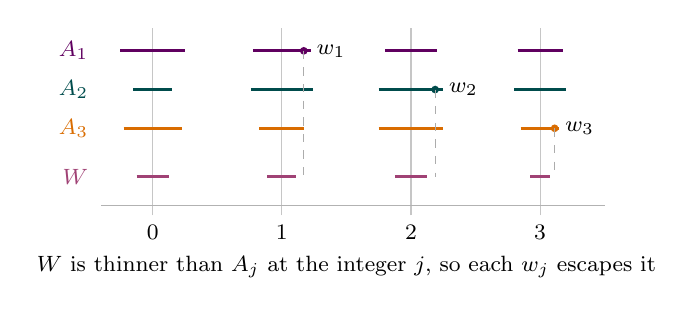
\begin{tikzpicture}[scale=0.82]
\foreach \x in {0,2,4,6} { \draw[gray!45] (\x,-0.15) -- (\x,2.75); }
\draw[gray!60] (-0.8,0) -- (7,0);
\foreach \x/\l in {0/0,2/1,4/2,6/3} { \node[font=\footnotesize,below] at (\x,-0.15) {$\l$}; }
\foreach \i/\a in {0/0.5,2/0.45,4/0.4,6/0.35} { \draw[violet!75!black,very thick] (\i-\a,2.4) -- (\i+\a,2.4); }
\foreach \i/\a in {0/0.3,2/0.48,4/0.5,6/0.4} { \draw[teal!60!black,very thick] (\i-\a,1.8) -- (\i+\a,1.8); }
\foreach \i/\a in {0/0.45,2/0.35,4/0.5,6/0.3} { \draw[orange!85!black,very thick] (\i-\a,1.2) -- (\i+\a,1.2); }
\foreach \i/\a in {0/0.25,2/0.225,4/0.25,6/0.15} { \draw[magenta!60!black,very thick] (\i-\a,0.45) -- (\i+\a,0.45); }
\node[violet!75!black,font=\footnotesize,anchor=east] at (-0.85,2.4) {$A_1$};
\node[teal!60!black,font=\footnotesize,anchor=east] at (-0.85,1.8) {$A_2$};
\node[orange!85!black,font=\footnotesize,anchor=east] at (-0.85,1.2) {$A_3$};
\node[magenta!60!black,font=\footnotesize,anchor=east] at (-0.85,0.45) {$W$};
\fill[violet!75!black] (2.34,2.4) circle (1.7pt);
\fill[teal!60!black] (4.375,1.8) circle (1.7pt);
\fill[orange!85!black] (6.225,1.2) circle (1.7pt);
\draw[dashed,gray!65] (2.34,2.4) -- (2.34,0.45);
\draw[dashed,gray!65] (4.375,1.8) -- (4.375,0.45);
\draw[dashed,gray!65] (6.225,1.2) -- (6.225,0.45);
\node[font=\footnotesize,anchor=west,inner sep=1.5pt] at (2.47,2.4) {$w_1$};
\node[font=\footnotesize,anchor=west,inner sep=1.5pt] at (4.52,1.8) {$w_2$};
\node[font=\footnotesize,anchor=west,inner sep=1.5pt] at (6.32,1.2) {$w_3$};
\node[font=\footnotesize] at (3,-0.95) {$W$ is thinner than $A_j$ at the integer $j$, so each $w_j$ escapes it};
\end{tikzpicture}
